\newpage
\chapter{Design del Software}
\section{Scema del Database e Modello di Dominio}
Il \textbf{livello di persistenza} è gestito da Spring Data JBA, che tramite Hibernate mappa le classi Java sulle tabelle del database PostgreSQL 
\subsection{Class Diagram del database}
\begin{figure}[ht]
    \centering
    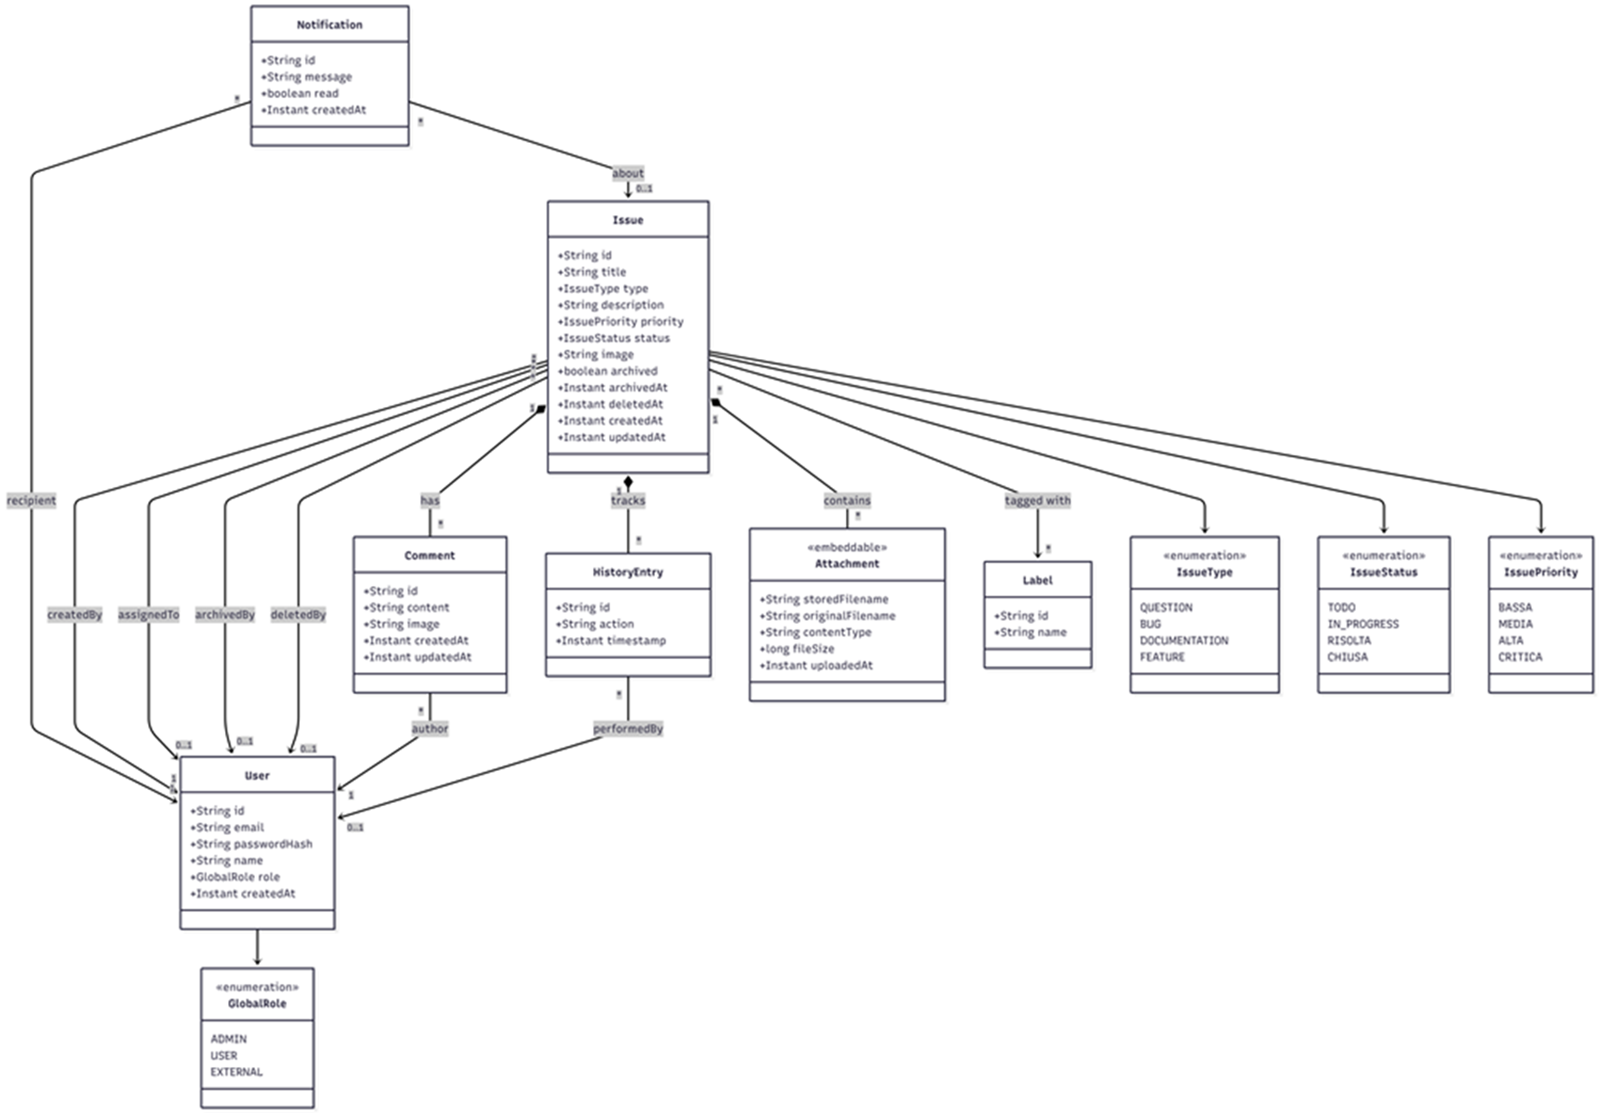
\includegraphics[width=0.75\linewidth]{ERINGSW.png}
    \caption{Class Diagram del database}
\end{figure}

\subsection{Descrizione entità}
\begin{itemize}[itemsep=2pt]
    \item \textbf{User:} Rappresenta un utente registrato nel sistema, al suo interno contiene: email nome, hash password, la data di creazione e il \textit{GlobalRole} associato
    \item \textbf{Issue:} Si tratta della task, bug, o funzionalità tracciata dal sistema. contiene data come: titolo, descrizione testuale, tipo, priorità, stato e informazioni temporali
    \item \textbf{Comment:} Una risposta testuale che può includere un'immagine, gestisce la conversazione di un singolo problema
    \item \textbf{Label:} Gestisce le etichette che possono essere assegnate ai task. Possiede un nome univoco nel database
    \item \textbf{HistoryEntity:} Ha lo scopo di storico modifiche, memorizzando le azioni effettuate dagli User e il timestamp in cui si è verificata 
    \item \textbf{Notification:} Rappresenta un messaggio di avviso da parte del sistema rivolto a un User. Contiene il messaggio di notifica, data di emissione e una flag di lettura 
\end{itemize}

\subsection{Descrizione Relazioni}
\begin{itemize}[itemsep=2pt]
    \item \textbf{Issue - User (Reporter):} associazione \textbf{* a 1} che identifica l'User che ha creato la segnalazione 
    \item \textbf{Issue - User (Assegnatario):} associazione \textbf{* a 1} che identifica l'User a cui è stata affidata la risoluzione di una segnalazione
    \item \textbf{Issue – User (Archiviatore):} associazione \textbf{* a 1} che indica l'User (amministratore) che ha archiviato la segnalazione
    \item \textbf{Issue - Label (Etichetta):} assosciazione \textbf{* a *} che permette di categorizzare una Issue a più Label, e di applicare lo stesso Label a più Issues diverse
    \item \textbf{Comment - User (Autore):} associazione \textbf{* a 1} che collega un commento all'User che l'ha creato
    \item \textbf{Comment - Issue (Riferimento):} assosciazione \textbf{* a 1} che collega 1 o più commenti alle Issue di appartenenza
    \item \textbf{Notification - User (Destinatario):} associazione \textbf{* a 1} che associa l'avviso di sistema all'User che deve riceverlo
    \item \textbf{Notification - Issue (Sorgente):} associazione \textbf{* a 1} opazionale, quale evento ha generato la segnalazione
    \item \textbf{HistoryEntry - Issue (Tracciamento):} associazione \textbf{* a 1} che collega vari storici all'Issue che ha subito variazioni nel corso del tempo
    \item \textbf{HystoryEntry - User (Esecutore):} associazione \textbf{* a 1} che indica l'User responsabile della modifica registrata nello storico
\end{itemize}

\newpage

\section{Organizzazione Architetturale dei Package}
\subsection{Package Diagram}
\begin{figure}[h]
    \centering
    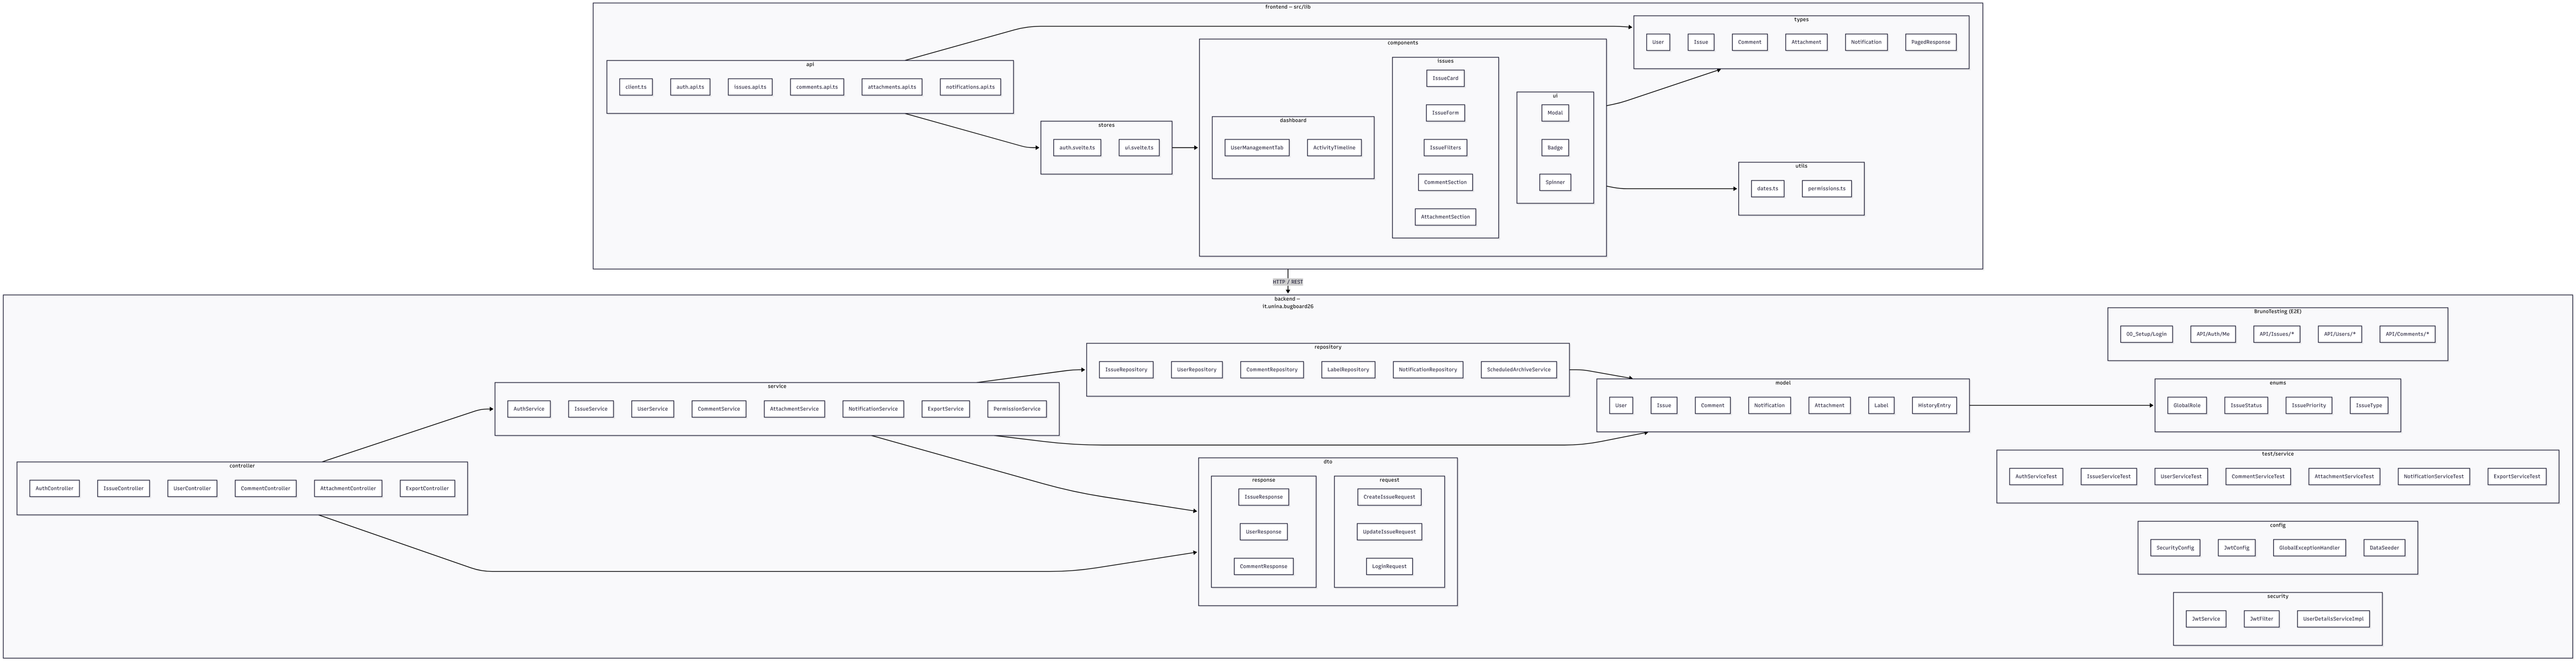
\includegraphics[width=1\linewidth]{package.png}
    \caption{Package diagram}
\end{figure}
Il progetto adotta una suddivisione in package (\textbf{Layered Architecture}) per separare le responsabilità e facilitarne la manutenzione
L'architettura del sistema è suddivisa in due aree principali che comunicano fra loro: \textbf{Backend(api)} e \textbf{Frontend(web)} 

\subsection{Backend (it.unina.bugboard26)}
Racchiude tutta la logica applicativa lato server. è strutturato seguendo la logica architetturale a strati:
\begin{itemize}
    \item \texttt{controller}: Rappresenta lo stato di presentazione delle api; riceve HTTP request dal client, delegando poi l'elaborazione allo s  trato successivo
    \item \texttt{service}: Esegue operazioni complesse, verifica permessi e gestisce i dati prima di passasrli al database o controller
    \item \texttt{repository}: Gestisce lo stato di persistenza: comprende i metodi per interrogare e manipolare i dati del database, usando Spring Data JPA per astrarre le query
    \item \texttt{model}: contiene le entità del dominio, classi che mappano esternamente le tabelle del database
    \item \texttt{dto(Data Transfer Object)}: Raccoglie gli oggetti utilizzati per trasferire i dati tra client e server, nascondendo la struttura interna del database 
    \item \texttt{security}: Si occupa della logica di autenticazione e autorizzazione, gestendo i filtri per i token JWT e l'integrità degli accessi
    \item \texttt{config}: Si occupa di raggruppare le configurazioni globali del sistema, quali eccezioni o configurazioni di sicurezza
    \item \texttt{enums}: Raccoglie i tipi enumerati condivisi a tutto il backend
\end{itemize}

\subsection{Frontend (web)}
Il package descritto riguarda l'organizzazione del codice del client web
\begin{itemize}
    \item \texttt{routes}: Gestisce il sistema di navigazione, associando gli URL alle pagine visibili dall'utente
    \item \texttt{lib/components}: Raggruppa gli elementi visivi rutilizzabili dall'UI, quali bottoni, modali, schede dei task e barre di navigazione.
    \item \texttt{lib/api}: Si occupa di comunicare con l'esterno. Contiene i client REST che effettuano le chiamate HTTP verso il backend
    \item \texttt{lib/stores}: Gestisce lo stato globale dell'applicazione dal lato client
    \item \texttt{lib/utils}: Fornisce funzioni di supporto, come la formattazione di date o permessi lato client
\end{itemize}

\subsection{Il flusso delle Dipendenze}
Il diagramma contiene regole di dipendenza usate per evitare accoppiamenti errati:
\begin{itemize}
    \item \textbf{Tra Macro-Package:} il pacchetto \texttt{lib/api} situato nel Frontend dipende interamente dai \texttt{controller} nel backend, comunicando tramite protocollo HTTP
    \item \textbf{Nel Backend:} La comunicazione è solo top-down. \texttt{controller} dipende da \texttt{service} e dai \texttt{dto}. il \texttt{service} dipende dal \texttt{repository} e \texttt{model}, mentre il \texttt{repository} unicamente dal \texttt{model}.
\end{itemize}
\subsection{Design Pattern applicati}
\begin{enumerate}
    \item \textbf{Model-View-Controller (MVC):} Usato per API RESTful. Il \textit{model} è rappresentato dalle entità JPA, il \textit{Controller} intercetta le richieste di rete, la \textit{View} è la struttura JSON rimandata al frontend
    \item \textbf{DTO (Data Transfer Object):} Applicato per isolare lo schema del database dai dati scambiati in rete
    \item \textbf{Repository Pattern:} Passa a Hibernate la traduzione delle query SQL
    \item \textbf{Dependency Injection:} Presente nativamenete dal framework Spring, permette ai componenti (es. Service) di dichiarare le dependencies (es. Repository) usando il costruttore, che poi verranno iniettate a runtime dal framework
\end{enumerate}

\newpage

\section{Sequence Diagrams}
I \textbf{Sequence Diagrams} modellano il comportamento del sistema, illustrando l'ordine delle interazioni tra attori esterni e componenti dell'architettura durante l'esecuzione del programma

\subsection{Sequence Diagram: User Login}
\begin{figure}[H]
    \centering
    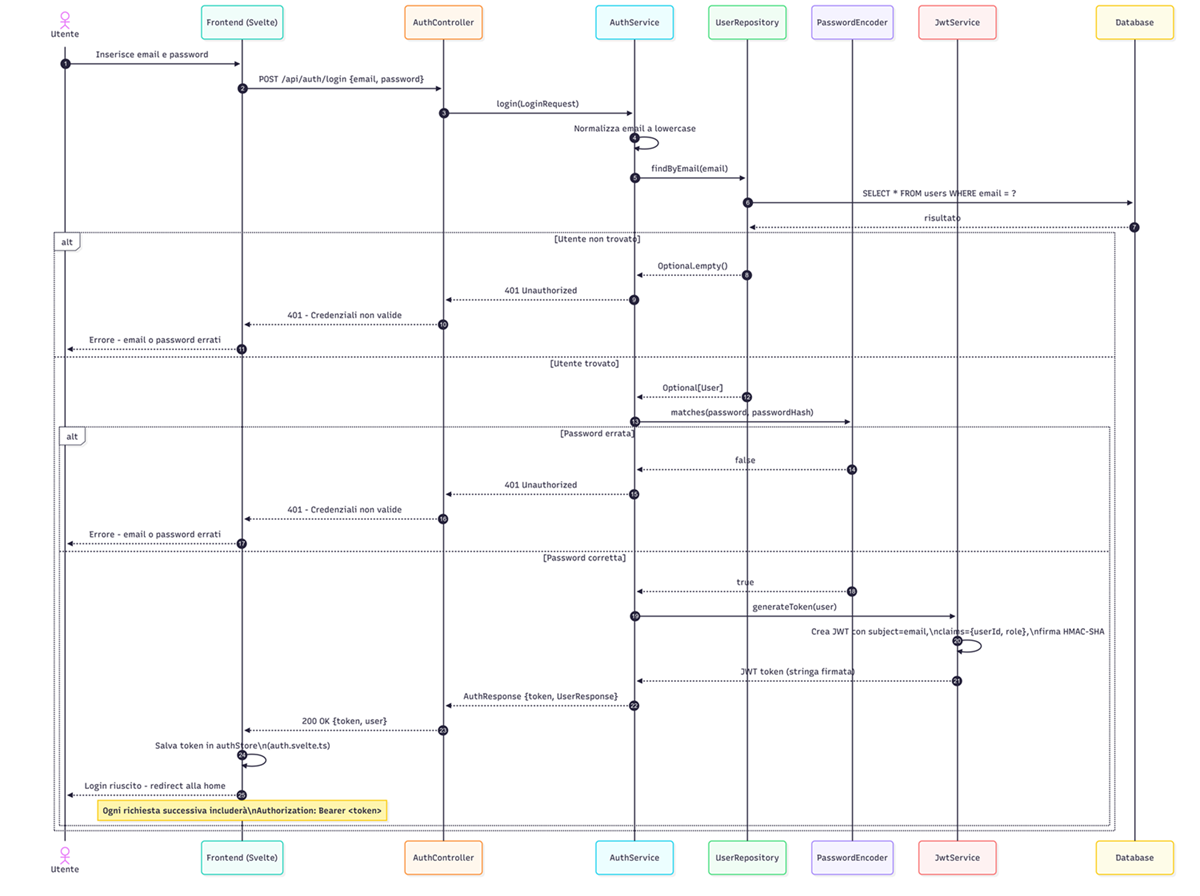
\includegraphics[width=0.7\linewidth]{sd_userauth.png}
    \caption{Sequence diagram Autenticazione Utente}
\end{figure}

Questo digramma descrive il flusso di verifica d'identità di un operatore, e in seguito la generazione del token crittografico per le sessioni \textit{stateless}

\textbf{Attori e componenti:}
\begin{itemize}
    \item \textbf{User:} L'essere umano che interagisce col sistema
    \item \textbf{User Interface:} frontend svilupptato in SvelteKit
    \item \textbf{AuthController:} Il punto di ingresso delle API esposte da Spring Boot
    \item \textbf{AuthService/JWTService:} I moduli contenenti la logica di validazione e crittografia
    \item \textbf{Database:} Il modulo di persistenza dove vengono conservati i dati (PostgreSQL)
\end{itemize}
\textbf{Flusso degli eventi:}
\begin{enumerate}
    \item User inserisce le proprie credenziali nel login module dell'UI
    \item L'applicazione client crea una richiest HTTP POST indirizzata all'APi di autenticazione, incapsulando i dati nel DTO \texttt{LoginRequest}
    \item L'\texttt{AuthController} riceve la richiesta, esegue una validazione della sintassie la delega al livello successivo richiamando l'\texttt{AuthService}
    \item l'\texttt{AuthService} interroga il database attraverso lo \texttt{UserRepository} cercando un account che corrisponda all'email fornito
    \item Il Database restituisce l'entità utente che comprende l'hash crittografato della keyword
    \item L'\texttt{AuthService} verifica la corrispondenza tra password in chiaro e l'hash salvato usando l'algoritmo BCrypt
    \item Se l'esito è positivom il modulo JwtService genera un JSON Web Token firmato, incluso di privilegi di GlobalRole utente
    \item Il server manda un HTTP Code 200 (success) e restituisce il JWT in un ODT AuthResponse
    \item L'UI salva il token nello storage locale e reindirizza lo User alla dashboard progetti
\end{enumerate}
\newpage
\subsection{Sequence Diagram: Creazione Segnalazione Bug/Issue}
\begin{figure}[ht]
    \centering
    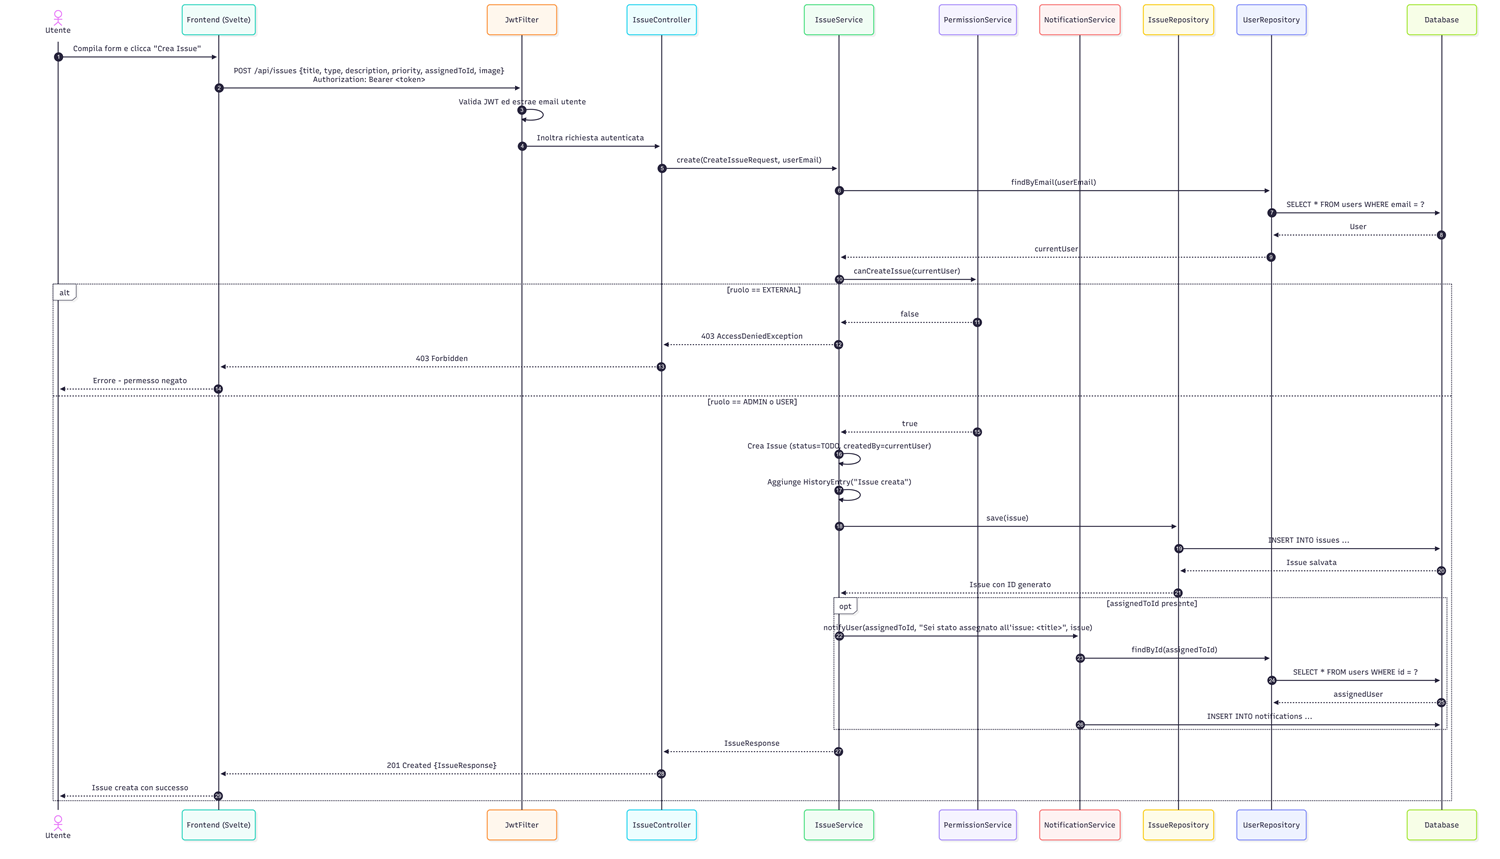
\includegraphics[width=0.7\linewidth]{sd_creazbug.png}
    \caption{Sequence Diagram Creazione Segnalazione Bug/Issue}
\end{figure}
Questo scenario riguarda il percorso di inserimento di una Issue o Bug all'interno del sistema, analizzando il meccanismo di autorizzazione previo all'aggiunta

\textbf{Attori e Componenti:}

\begin{itemize}
    \item \textbf{User Autenticato:} Operatore provvisto di JWT valido e privilegi
    \item \textbf{User Interface:} Componente di rendering della form
    \item \textbf{JwtFilter:} filtro di sicurezza apparente al framework Spring Security
    \item \textbf{Issue Controller:} Controller segnalazioni delle richieste per l'entità Issue
    \item \textbf{IssueService:} Modulo gestore della logica di business
    \item \textbf{Database:} Modulo di persistenza
\end{itemize}

\textbf{Flusso degli Eventi:}
\begin{enumerate}
    \item L'Utente autenticato compila il modulo di segnalazione nell'UI, specificando titolo, descrizione, tipo, priorità, dunque salva
    \item L'app web SvelteKit invia una richiesta HTTP POST all'API. La richiesta include: JWT nell'header di autenticazione e payload strutturato come \texttt{CreateIssueRequest} 
    \item La richiesta viene intercettata dal \texttt{JwtFilter}, che estrare il JWT, ne valida la firma e ricostruisce l'identità e il ruolo dell'operatore
    \item Una volta superato il filter, l'\texttt{IssueController} decodifica la richiesta e la passa all'\texttt{IssueService}
    \item L'\texttt{IssueService} convalida le regole di dominio (verificando che il ruolo dell'utente garantisca la creazione di Issues) e crea una nuova entità issue. impiostandone lo stato iniziale predefinito (TODO)
    \item Tramite l'\texttt{IssueRepository} Il servizio comunica con il Database, richiedendone la persistenza delle entità
    \item Il Database esegue l'operazione \texttt{Insert} e restituisce l'identità compresa di ID univoo generato e il timestamp
    \item L'\texttt{IssueController} mappa l'entità salvata in un response DTO \texttt{IssueResponse} e lo invia al client con un codice HTTP 201 (Creato con successo)
    \item L'UI riceve la conferma, mostra un toast di creazione avvenuta con successo e aggiorna la lista delle segnalazioni        
\end{enumerate}